\documentclass{article}
\usepackage{amsthm,amsfonts}
\usepackage{graphicx}

%\input{pat.tex}
\newtheorem{lem}{Lemma}
\newtheorem{thm}{Theorem}
\newtheorem{prop}{Proposition}
\newcommand{\cn}{\mathsf{cr}}
\newcommand{\dn}{\mathsf{dn}}


\begin{document}




\begin{thm}
For any outerplanar graph $G$, $\dn(G)\le 3$.
\end{thm}

\begin{proof} 

Without loss of generality, we may assume that $G$ is maximal
outerplanar.  We call each cycle of length 3 in $G$ a \emph{triangle}
of $G$.  A drawing of $G$ using only three edge lengths is obtained as
follows: Consider the \emph{face-edge dual} $T$ of $G$ whose vertices
are the triangles of $G$ and in which two triangles are adjacent iff
they share an edge.  It is well-known that, since $G$ is maximal
outerplanar, $T$ is a binary tree. Select an arbitrary triangle of
$G$ to act as the root of $T$ and call this triangle the \emph{root
triangle}.

We locate the root triangle's vertices at the points $p_0=(0,0)$,
$p_1=(1,0)$ and some point $p_2=(x,y)$ in the unit square $[0,1]^2$ whose
coordinates will be specified later.  Consider any triangle $uvw$ of
$G$ that is not the root triangle and assume (recursively) that the
three vertices of the parent $uvw'$ of $uvw$ have already been
assigned locations.  The location of $w$ is then obtained by
reflecting $w'$ through the line containing $u$ and $v$.  In this way,
each vertex of $G$ is assigned a location that is determined entirely
by the point $p_2$.

We will show that there is a choice of the point $p_2$ that results in
a drawing of $G$ by showing that, for any vertex-edge pair $(v_i,e_j)$
the set of choices of $p_2$ for which $v_i$ is located in $e_j$ is a
1-dimensional set.\footnote{A set $S$ of points in the plane is a
2-dimensional set if it contains a disk of positive radius.  If $S$ is
not 2-dimensional but contains a finite curve then $S$ is
1-dimensional.  If $S$ is non-empty but is neither 1-dimensional nor
2-dimensional then $S$ is $0$-dimensional.} Thus, the set of choices
of $p_2$ for which some vertex lies on some edge is a finite union of
1-dimensional sets, and is therefore also 1-dimensional.  However,
$p_2$ can be selected to be any point in $[0,1]^2$, a
2-dimensional set, so it suffices to select any $p_2$ that is not in
this 1-dimensional set.

Note that, since the root triangle is selected arbitrarily, we may
assume that $e_j$ is an edge of the root triangle.  We distinguish
between two cases.  In the first case, $e_j$ is the segment $p_0p_1$,
i.e., the bottom edge of the root triangle.  Let $f:[0,1]^2\mapsto
\mathbb{R}^2$ be the function that defines the location of $v_i$ given
the location of $p_2$.  The codomain (range) of $f$ is a 2-dimensional
set and the intersection of the segment $p_0p_1$ with this set is a
1-dimensional set. The preimage of $p_0p_1$ in $f$ is a 1-dimensional
subset of $[0,1]^2$, as required.

Next we consider the case where $e_j$ is one of the other two edges of
the root triangle, say the segment $p_0p_2$.  In this case,
consider the representation of $p_2$ using polar coordinates
$(\ell,\theta)$ where $\ell=\|p_0p_2\|$ and $\theta=\angle p_1p_0p_2$.
By a change of coordinates, we may assume that the segment $p_0p_2$
is contained in the $x$-axis so that the root triangle has vertices
$p_0=(0,0)$, $p_2=(-\ell,0)$ and $p_1=(-\cos\theta,\sin\theta)$.
Again, the parameters $\ell$ and $\theta$ can be selected from a
2-dimensional set and there is a function $g$ that defines the
location of $v_i$ given $\ell$ and $\theta$.  Note that, if
$g(\ell,\theta)$ is contained in the segment $p_0p_2$ then
$g(\ell,\theta)$ is on the $x$ axis.  The preimage of the $x$-axis in
$g$ is a 1-dimensional subset of the 2-dimensional set that describes
all valid choices of $\ell$ and $\theta$ and this 
corresponds to a 1-dimensional subset of $[0,1]^2$ which describes all
valid choices of $x$ and $y$, as required.
\end{proof}

Note that, without some further ideas, it is not possible to
generalize the above proof to show that $\dn(G)\le 2$ if $G$ is
outerplanar.  In particular, with only two distance classes, all
triangles of $G$ are isosceles triangles defined by a single parameter
$\alpha$ that measures the angle at the apex.  In this case, the range
of the function $g$ is a 1-dimensional set and this set can coincide
with the line containing $[p_0,p_2]$.  The example in the figure below
shows an example where this occurs.  In this example, any choice
of $\alpha$ in the interval $[0,\pi/6]$ results in the vertex $v_i$ being
embedded on the segment $p_0p_2$.

\begin{tabular}{cccc}
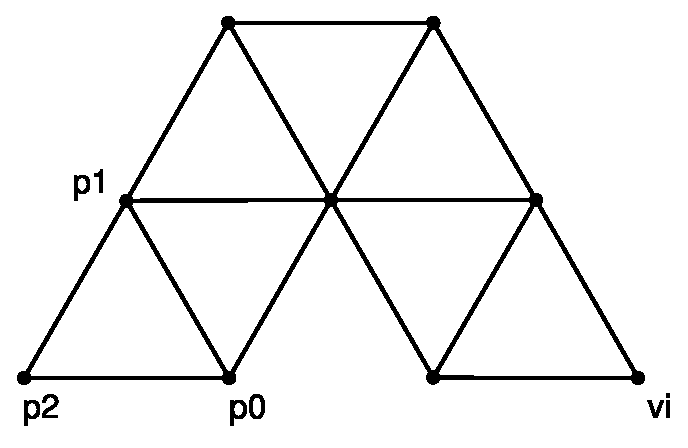
\includegraphics[scale=.30]{no2-1} &
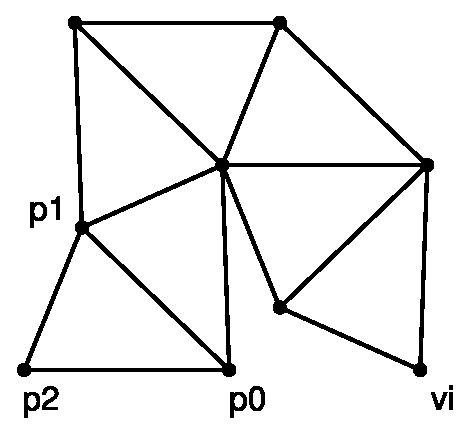
\includegraphics[scale=.30]{no2-2} &
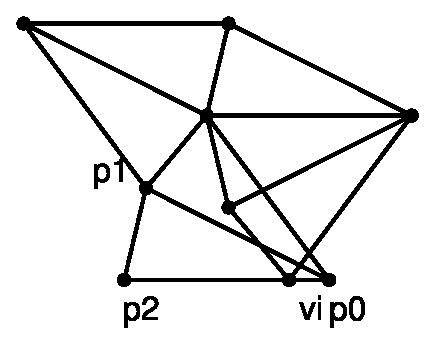
\includegraphics[scale=.30]{no2-3} &
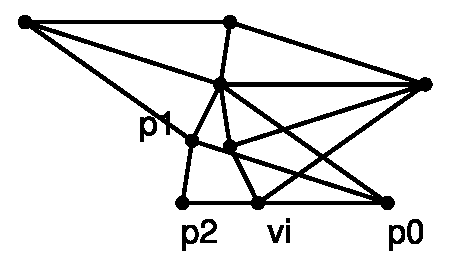
\includegraphics[scale=.30]{no2-4} 
\end{tabular}

It is easy to observe that there are outerplanar graphs with distance
number greater than 1.  Consider for example the graph comprised of
one degree-6 vertex adjacent to each vertex of a path of length 6. For
edge-maximal outerplanar graphs, in fact for all weak planar
triangulations\footnote{A planar graph is \emph{weakly triangulated}
if it has an embedding where the edges on the unbounded face form a
cycle and the edges of the bounded faces form 3-cycles.} we can decide
if they have distance number 1.

\begin{prop} A weak planar triangulation $G$ has distance number 1 if
and only if it is a subgraph of the triangular grid.\footnote{The
triangular grid is the infinite graph with vertex set 
$V=\{(i+j/2,j\sqrt{3}/2): i,j\in\mathbb{Z}\}$ and in which two vertices are
adjacent iff the Euclidean distance between them is 1.}  Furtermore,
testing if a weak planar triangulation has distance number 1 can be
done in $O(n)$ time.  \end{prop}

\begin{proof}
The characterization part of the proposition follows immediately from
the fact that the assignment of vertex locations to the vertices of
$G$ is unique, up to the choice of location of one triangle of $G$.

To obtain an efficient algorithm for testing if $G$ is a subgraph of
the triangular grid  we can compute any spanning tree $T$ of the
face-edge dual of $G$.  By assigning the root of $T$ to be a grid
triangle adjacent to the origin and traversing $T$ we can, in linear
time, obtain locations for all vertices of $G$.  This provides vertex
locations for $G$ such that each vertex is located on a point of the
triangular grid.  All that remains to check is that each edge has unit
length and that no two vertices are assigned to the same grid point.

Checking that each edge of $G$ has unit length is trivially done in
constant time per edge.  To check that no two vertices of $G$ are
assigned to the same grid point we observe that the points of the
triangular grid can be uniquely indexed by pairs of integers (see the
footnote).  Furthermore, for the vertex locations of $G$ these
integers are in the set $\{-n,\ldots,n\}$.  Thus, using radix sort we
can, in $O(n)$ time, sort the vertices of $G$ by their location to
determine if any two vertices are assigned the same location.
\end{proof}

\end{document}
